\section{Arithmetic}

\subsection{Floating Point Numbers}
\begin{figure}[H]
\centering
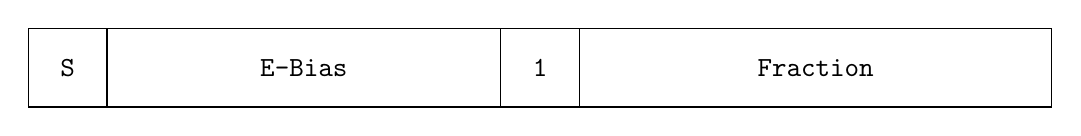
\begin{tikzpicture}
    \draw (0,0) -- (13,0);
    \draw (0,1) -- (13,1);
    \foreach \x in {0,1,6,7,13}
        \draw (\x,0) -- (\x,1);
    \node at (0.5,0.5) {\texttt{S}};
    \node at (3.5,0.5) {\texttt{E-Bias}};
    \node at (6.5,0.5) {\texttt{1}};
    \node at (10,0.5) {\texttt{Fraction}};
\end{tikzpicture}    
\end{figure}

\subsection{Converting Decimal to Floating Point}
\begin{itemize}
    \item Convert integer part to binary.
    \item Convert fractional part by multiplying by 2 each time and shifting the decimal point right one until there is no fractional part left.
    \item Append $2^0$ to the end of the number, this has no effect.
    \item Normalise the number by moving your binary point to one bit from the left (be sure to adjust exponent accordingly).
    \item The fractional field is then the bits to the right of the binary point. Pad the remaining bits with 0's, so for IEEE 32-bit floats the fractional field has 23 bits.
    \item Add an exponent bias of $2^{k-1}-1$ where $k$ is the number of bits in the exponent field. For IEEE 32-bit float, $k=8$, so the bias is $2^{8-1}-1=127$. 
    \item Set the sign bit as \texttt{1} if the number is negative, \texttt{0} otherwies.
\end{itemize}

\begin{framed}
\textbf{Convert 2.625 to our 8-bit floating point format.} \\ \par
Integer part, $2_{10}=10_{2}$. \\
Fraction part, 
\begin{align*}
    0.625\times 2=1.25 \quad \boxed{\mbox{\texttt{1}}} \\
    0.25\times 2=0.5 \quad \boxed{\mbox{\texttt{0}}} \\
    0.5\times 2=1.0 \quad \boxed{\mbox{\texttt{1}}}
\end{align*}
So, $0.625_{10}=0.101_2$ and $2.625_{10}=10.101_2$.
\begin{align*}
    \mbox{Add exponent part, } & 10.101_2 = 10.101_2 \times 2^0 \\
    \mbox{Normalise, } & 10.101_2 \times 2^0 = 1.0101_2 \times 2^1 \\
    \mbox{Fractional field, } & 0101_2 \\
    \mbox{Exponent, } & 1+127=128_{10}=10000000_{2} \\
    \mbox{Sign bit, } & 0
\end{align*}
$\therefore 2.625_{10} = \boxed{0}\boxed{10000000}\boxed{01010000000000000000000}$
\end{framed}

\subsection{Adders}
\subsubsection{Ripple Adder}
An $n$-bit ripple adder is constructed by cascading $n$ full adder cells. The size of this is proportional to the number of cells you have. However since cell $n+1$ takes the carry bit from the previous addition the delay will also be proportional to $n$.

\begin{figure}[H]
    \centering
    \includegraphics[width=0.5\textwidth]{img/ripple-adder}
    \caption{Cascading full adders.}
\end{figure}

\subsubsection{Carry--Lookahead Adder}
A carry-lookahead adder works by calculating the carry of each adding stage separately. This makes the delay constant regardless of the number of bits but also  low (only chip propagation delays). However each stage is geometrically larger than the previous and it is said that $\mbox{size} \propto n^2$.

% TODO: carry-lookahead schematic

\subsection{Multicycling Addition}
% TODO: multicycling addition
\subsection{Floating Point Addition/Subtraction}
% TODO: floating point +/-
\subsection{Floating Point Multiplication/Division}
% TODO: floating point */÷

\subsection{Microcoded Operations}
Microcode allows us to add simple functionality that isn't already present in hardware. Below is an example of a 32-bit unsigned square root in C code.

\begin{minted}{c}
int fn sqrt(int val)
{
    int mask = 0x00008000;
    int best = 0x00000000;
    if (val <= 0) return 0;
    while (mask != 0) {
        if ((best+mask^2) <= val) best |= mask;
        mask >>= 1;
    }
    return (int)best;
}
\end{minted}





